\chapter{Conception architecturale}
\label{chap:archi}

La pile protocolaire en cinq couches qui structure la lecture de BCaaS a été présentée au
chapitre~\ref{chap:analogie} (figure~\ref{fig:pile}). Le présent chapitre se concentre sur
les choix d'architecture logicielle qui la concrétisent : l'architecture hexagonale, le
monolithe modulaire et l'organisation en packages.

\section{Architecture hexagonale et DDD}

BCaaS adopte une architecture hexagonale (ports et adaptateurs) combinée au Domain-Driven
Design. Le domaine métier (entités, règles, machines à états) est isolé au centre ;
les détails techniques (persistance JPA, exposition REST, messagerie) sont relégués aux
adaptateurs périphériques. Cette organisation garantit que le cœur métier ne dépend
d'aucune technologie particulière, condition d'une évolution ultérieure sereine.

Concrètement, le flux d'une requête traverse les couches applicatives suivantes :
\[
\text{Controller (REST)} \to \text{Service (domaine)} \to \text{Repository (JPA)} \to
\text{Base de données},
\]
les DTO assurant le découplage entre la représentation exposée et les entités persistées.

\section{Monolithe modulaire « microservices-ready »}

Conformément aux contraintes du sujet, BCaaS est un \textbf{monolithe modulaire} : les
modules métier (acteurs, métiers, catalogues, demandes, factures, audit, analytique) sont
organisés en packages cohérents et communiquent par appels en mémoire. Ce choix simplifie
le déploiement et la coordination initiale tout en préservant des frontières nettes : les
modules pourront, à terme, être extraits en microservices déployés indépendamment, sans
réécrire le domaine (perspective détaillée au chapitre~\ref{chap:perspectives}).

%\figplaceholder{Architecture logique de BCaaS : API %Gateway (Auth JWT, routing,
%%X-Tenant-ID) au-dessus des modules métier (Actor, %Business, Service Catalogue, Service
%Request, Invoice, Resource, Media, Notification, %Audit, Analytics), reposant sur
%l'infrastructure (PostgreSQL, Redis, bus %d'événements).}{6.5cm}

\begin{figure}[H]
    \centering
    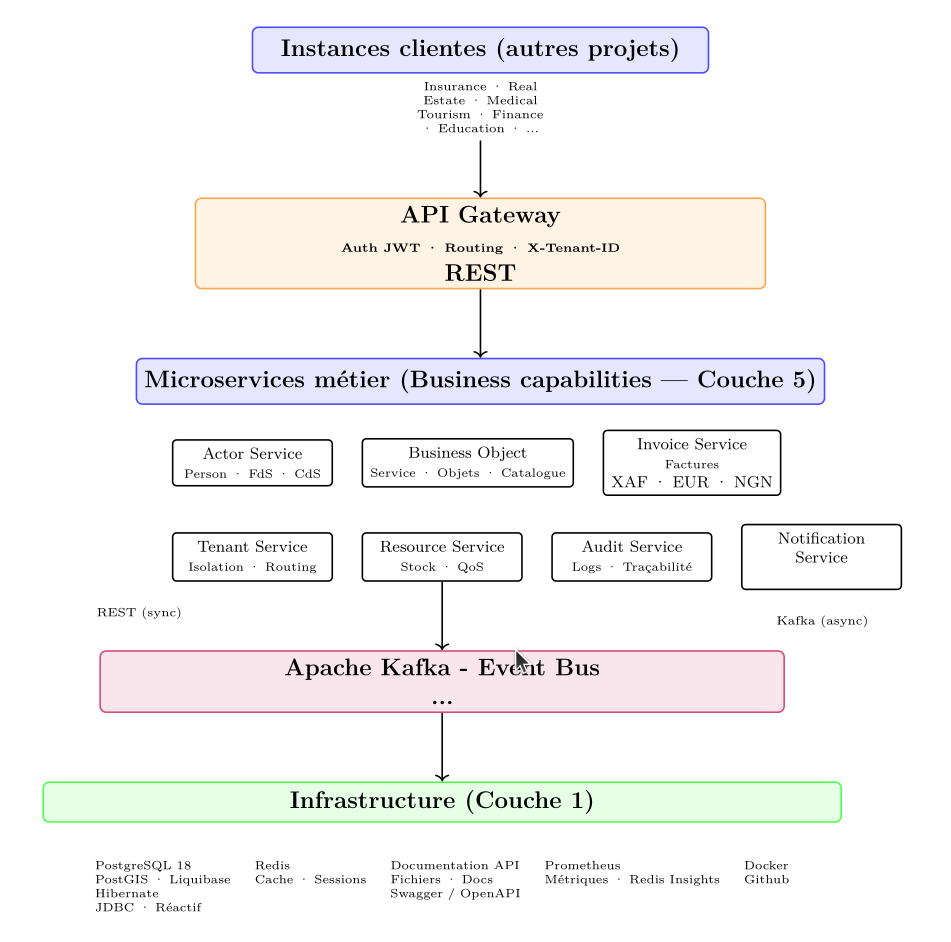
\includegraphics[width=0.8\linewidth]{chapitres/Capture d’écran du 2026-06-16 08-18-23.png}
    \captionof{figure}{Architecture logique de BCaaS}
    \label{fig:placeholder}
\end{figure}


\section{Diagramme de packages}

L'organisation en packages reflète les domaines fonctionnels : authentification, gestion
des acteurs, gestion des métiers, gestion des services, gestion des médias, gestion des
ressources et gestion des factures. Chaque package porte des responsabilités bien
délimitées, ce qui facilite l'évolution indépendante des règles métier et des mécanismes

\paragraph{Tenant}
L'acteur Tenant suggère une architecture multi-tenant, où chaque client (organisation ou locataire) dispose de sa propre isolation des données et configurations. Ce package agit probablement comme un contexte global d'exécution permettant aux autres modules de fonctionner de manière isolée par tenant.

\paragraph{Authentification et gestion des acteurs}
Le package AUTHENTIFICATION gère les processus d'identification et de vérification des tenants. Il interagit directement avec GESTION DES ACTEURS qui centralise la définition, les rôles et les permissions des différentes entités utilisatrices (administrateurs, clients, fournisseurs, etc.). Cette séparation permet de dissocier le mécanisme technique d'authentification de la gestion administrative des profils.

\paragraph{Gestion des business et services}
Les packages GESTION DES BUSINESS et GESTION DES SERVICES couvrent le cœur métier. Le premier traite des règles propres à l'activité de l'entreprise, tandis que le second coordonne l'information, l'orchestration ou la souscription aux services proposés. Leur découpage facilite l'évolution indépendante des règles métier et des mécanismes de service.

\paragraph{Gestion des médias, ressources et factures}
Le package GESTION DES MEDIA est dédié aux contenus multimédias (images, vidéos, documents). GESTION DES RESSOURCES supervise les actifs techniques ou matériels nécessaires au fonctionnement (serveurs, licences, matériel, équipements). Enfin, GESTION DES FACTURES assure la chaîne de facturation, de la génération des factures au suivi des paiements.

%\figplaceholder{Diagramme de packages UML : %AUTHENTIFICATION, GESTION DES ACTEURS, GESTION
%DES BUSINESS, GESTION DES SERVICES, GESTION DES MEDIA, %GESTION DES RESSOURCES, GESTION DES
%FACTURES, sous le contexte multi-tenant.}{6.5cm}

\begin{figure}[H]
    \centering
    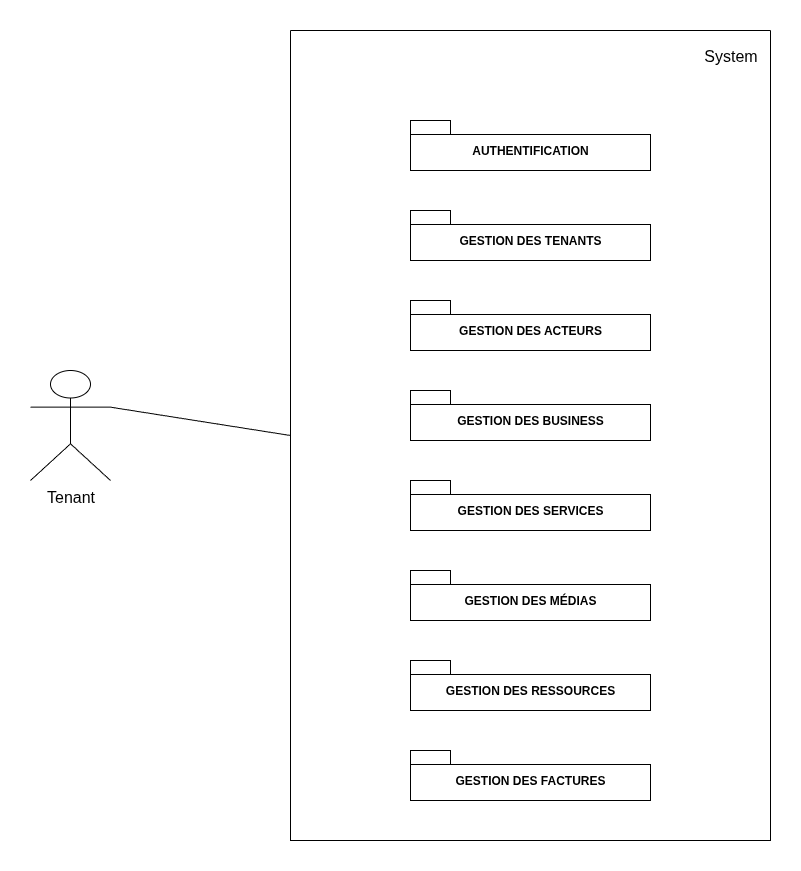
\includegraphics[width=0.8\linewidth]{chapitres/package.drawio.png}
   \captionof{figure}{Diagramme de packages de l'architecture du système}
    \label{fig:placeholder}
\end{figure}
\label{fig:packages}

